\documentclass[class=ctexart,crop=false]{standalone}

\usepackage{amsmath,amssymb,enumitem,empheq,tkz-euclide,
diagbox,wrapfig,pgfplots,geometry}
%\geometry{a4paper,scale=0.9}
\pgfplotsset{compat=newest}
%\usepgfplotslibrary{external}
%\tikzexternalize
\renewcommand\parallel{\mathrel{/\mskip-2.5mu/}}

\newcommand\px{\mathrel{/\mkern-5mu/}}  %平行
\newcommand\pxeq{\mathrel{\vcenter{     %平行且等于
\ialign{\hfil##\hfil\crcr
$\scriptstyle\px\!$\crcr
\noalign{\nointerlineskip\vskip1pt}$=$\crcr}}}}

%\setCJKmainfont{SimSun}       %设置西文字体为times new roman
%\setCJKsansfont{SimSun}             %设置中文字体为宋体
%\setCJKmonofont{STKaiti}
%\setsansfont{TeX Gyre Termes}            %设置typewriter family中文字体为楷体
%\setmonofont{TeX Gyre Termes}

\usetikzlibrary{calc,intersections,through,backgrounds,patterns}
\newcounter{para}
\newcommand\mypara{\par\refstepcounter{para}\thepara.\space}%设置typewriter family西文字体为times new roman
\newcommand*\circled[1]{\tikz[baseline=(char.base)]{
            \node[shape=circle,draw,inner sep=1pt] (char) {#1};}}

\newcommand{\rnum}[1]{\romannumeral #1}
\newcommand{\RNum}[1]{\uppercase\expandafter{\romannumeral #1\relax}}
\begin{document}
解:\\
\begin{enumerate}[label=(\arabic*)]
	\item
	      $ f(x)=\left\{\begin{aligned}
			      2-x & ,x \leqslant -2 \\
			      x-2 & ,x > 0
		      \end{aligned}\right.$\\
	      $ g(x)=\left\{\begin{aligned}
			      -4   & ,x \leqslant -1.5    \\
			      4x+2 & ,1.5<x \leqslant 0.5 \\
			      4    & ,x>0.5               \\
		      \end{aligned}\right.$\\
	      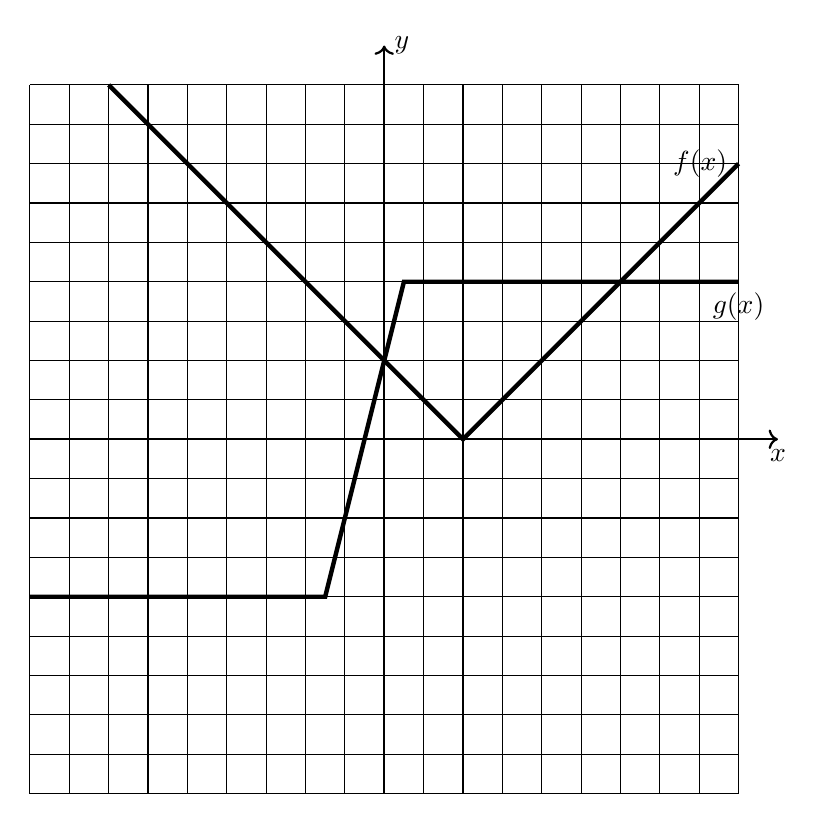
\begin{tikzpicture}[scale=0.5]
		      \draw[help lines,black] (-9,-9) grid (9,9); %网格线
		      \draw [->,thick] (-9,0)--(10,0) node[below] {$x$};
		      \draw [->,thick] (0,-9)--(0,10) node[right] {$y$};
		      \draw[ultra thick] (-7,9)--(2,0)--(9,7) node[left] {$f(x)$};
		      \draw[ultra thick] (-9,-4)--(-1.5,-4)--(0.5,4)--(9,4)node[below] {$g(x)$};
	      \end{tikzpicture}
	\item $f(x+a)$ 的图像为 $f(x)$ 向左移动a个单位\\
	      观察图像得知,若 $a<0$ 图像右移,$f(2-a)=0<4$ ,不满足题意
	      若左移,则需 $f(2-a)$ 在 $g(-0.5)$ 左侧,右支的$f(x_1)=4$ 在 $g(0.5)=4$ 左侧\\
	      $f(x)=4$ 时, $x=-2+a,6+a$\\
	      则$2-a \leqslant 0.5,6-a \leqslant 0.5$\\
	      综上, $a \geqslant 5.5$
\end{enumerate}
\end{document}